% Options for packages loaded elsewhere
\PassOptionsToPackage{unicode}{hyperref}
\PassOptionsToPackage{hyphens}{url}
%
\documentclass[
]{article}
\usepackage{amsmath,amssymb}
\usepackage{lmodern}
\usepackage{iftex}
\ifPDFTeX
  \usepackage[T1]{fontenc}
  \usepackage[utf8]{inputenc}
  \usepackage{textcomp} % provide euro and other symbols
\else % if luatex or xetex
  \usepackage{unicode-math}
  \defaultfontfeatures{Scale=MatchLowercase}
  \defaultfontfeatures[\rmfamily]{Ligatures=TeX,Scale=1}
\fi
% Use upquote if available, for straight quotes in verbatim environments
\IfFileExists{upquote.sty}{\usepackage{upquote}}{}
\IfFileExists{microtype.sty}{% use microtype if available
  \usepackage[]{microtype}
  \UseMicrotypeSet[protrusion]{basicmath} % disable protrusion for tt fonts
}{}
\makeatletter
\@ifundefined{KOMAClassName}{% if non-KOMA class
  \IfFileExists{parskip.sty}{%
    \usepackage{parskip}
  }{% else
    \setlength{\parindent}{0pt}
    \setlength{\parskip}{6pt plus 2pt minus 1pt}}
}{% if KOMA class
  \KOMAoptions{parskip=half}}
\makeatother
\usepackage{xcolor}
\IfFileExists{xurl.sty}{\usepackage{xurl}}{} % add URL line breaks if available
\IfFileExists{bookmark.sty}{\usepackage{bookmark}}{\usepackage{hyperref}}
\hypersetup{
  pdftitle={Natural regeneration of a tropical timber plantation},
  pdfauthor={Nicholas Medina},
  hidelinks,
  pdfcreator={LaTeX via pandoc}}
\urlstyle{same} % disable monospaced font for URLs
\usepackage[margin=1in]{geometry}
\usepackage{graphicx}
\makeatletter
\def\maxwidth{\ifdim\Gin@nat@width>\linewidth\linewidth\else\Gin@nat@width\fi}
\def\maxheight{\ifdim\Gin@nat@height>\textheight\textheight\else\Gin@nat@height\fi}
\makeatother
% Scale images if necessary, so that they will not overflow the page
% margins by default, and it is still possible to overwrite the defaults
% using explicit options in \includegraphics[width, height, ...]{}
\setkeys{Gin}{width=\maxwidth,height=\maxheight,keepaspectratio}
% Set default figure placement to htbp
\makeatletter
\def\fps@figure{htbp}
\makeatother
\setlength{\emergencystretch}{3em} % prevent overfull lines
\providecommand{\tightlist}{%
  \setlength{\itemsep}{0pt}\setlength{\parskip}{0pt}}
\setcounter{secnumdepth}{-\maxdimen} % remove section numbering
\newlength{\cslhangindent}
\setlength{\cslhangindent}{1.5em}
\newlength{\csllabelwidth}
\setlength{\csllabelwidth}{3em}
\newlength{\cslentryspacingunit} % times entry-spacing
\setlength{\cslentryspacingunit}{\parskip}
\newenvironment{CSLReferences}[2] % #1 hanging-ident, #2 entry spacing
 {% don't indent paragraphs
  \setlength{\parindent}{0pt}
  % turn on hanging indent if param 1 is 1
  \ifodd #1
  \let\oldpar\par
  \def\par{\hangindent=\cslhangindent\oldpar}
  \fi
  % set entry spacing
  \setlength{\parskip}{#2\cslentryspacingunit}
 }%
 {}
\usepackage{calc}
\newcommand{\CSLBlock}[1]{#1\hfill\break}
\newcommand{\CSLLeftMargin}[1]{\parbox[t]{\csllabelwidth}{#1}}
\newcommand{\CSLRightInline}[1]{\parbox[t]{\linewidth - \csllabelwidth}{#1}\break}
\newcommand{\CSLIndent}[1]{\hspace{\cslhangindent}#1}
\ifLuaTeX
  \usepackage{selnolig}  % disable illegal ligatures
\fi

\title{Natural regeneration of a tropical timber plantation}
\author{Nicholas Medina}
\date{}

\begin{document}
\maketitle

\hypertarget{outline}{%
\section{Outline}\label{outline}}

\begin{itemize}
\tightlist
\item
  Introduction
\item
  Methods
\item
  Results
\item
  Discussion
\end{itemize}

\hypertarget{iglobal-forests-are-regenerating-but-how}{%
\section{I--Global forests are regenerating, but
how?}\label{iglobal-forests-are-regenerating-but-how}}

\begin{itemize}
\item
  \textasciitilde Half of forests are tropical, and over half of all
  forests globally are secondary \emph{(FAO 2020)}
\item
  Services like timber and biodiversity depend on natural and managed
  regeneration patterns
\item
  Regeneration dynamics (e.g.~associated biodiversity) should be better
  understood to optimize sustainable management and service provision
\end{itemize}

\hypertarget{iforest-regeneration-is-overall-both-quick-and-inconsistent}{%
\section{I--Forest regeneration is overall both quick and
inconsistent}\label{iforest-regeneration-is-overall-both-quick-and-inconsistent}}

\begin{itemize}
\item
  Biomass recovers 90\% in 66 yrs \emph{(Poorter et al. 2016)}
\item
  Taxonomic richness recovers quickly \emph{(Rozendaal et al. 2019)}
\item
  Community composition may take centuries to recover, if at all
  \emph{(Norden et al. 2015)}
\end{itemize}

\hypertarget{ihabitat-edges-shape-regeneration}{%
\section{I--Habitat edges shape
regeneration}\label{ihabitat-edges-shape-regeneration}}

\begin{itemize}
\item
  70\% forests are \textless1 km from a habitat edge \emph{(Haddad et
  al. 2015)}
\item
  Edge effects reduce biodiversity 13 - 75\%

  \begin{itemize}
  \tightlist
  \item
    more so in small and isolated fragments
  \end{itemize}
\end{itemize}

\hypertarget{iedge-effects-may-differ-in-wet-tropical-plantations}{%
\section{I--Edge effects may differ in wet tropical
plantations}\label{iedge-effects-may-differ-in-wet-tropical-plantations}}

\begin{itemize}
\item
  7\% of global forests are planted and planted area has increased over
  last 30 yrs \emph{(FAO 2020)}

  \begin{itemize}
  \tightlist
  \item
    Often dense with fast-growing, shade-intolerant taxa
  \end{itemize}
\item
  Wet tropical forest regeneration tends to be light-limited, based on
  tree functional traits \emph{(Poorter et al. 2021)}
\item
  Existing plantation demography and shade may skew/buffer edge effects
  toward net positive instead of negative
\end{itemize}

\hypertarget{ithis-study}{%
\section{I--This study}\label{ithis-study}}

\begin{itemize}
\item
  Question -- How is wet tropical secondary forest regeneration affected
  by former plantation status and edges with road and primary forest?
\item
  Hypothesis --

  \begin{itemize}
  \item
    Former plantation status facilitates succession by allowing
    shade-intolerant taxa to grow better due to \textbf{denser canopies}
  \item
    Forest edges promotes regeneration by faciltating \textbf{dispersal}
    of shade-tolerant taxa
  \end{itemize}
\item
  Predictions -- Distance away from primary forest edge is associated
  with --

  \begin{itemize}
  \item
    lower stand biomass
  \item
    lower tree diversity
  \item
    lower shade-tolerant taxa
  \end{itemize}
\end{itemize}

\hypertarget{iistudy-site}{%
\section{II--Study site}\label{iistudy-site}}

\begin{itemize}
\item
  Wet tropical rainforest in Osa Peninsula, SW Costa Rica
\item
  20 ha plantation of dry forest timber, abandoned in
  \textasciitilde2003 into NRDC preserve
\item
  Area surrounded by primary forest on two sides and road on third
\end{itemize}

\hypertarget{iicensus-design}{%
\section{II--Census design}\label{iicensus-design}}

\begin{itemize}
\item
  Random stratified forest biomass inventory sampling design --

  \begin{itemize}
  \item
    divided 300 m range into six 50 m strata, from forest to road edge,
    using QGIS and ArcGIS
  \item
    30, 21 x 21 m plots randomly distributed, but quantity roughly
    proportional to stratum area
  \item
    All plots covered 1 ha total, 5\% of entire plantation
  \end{itemize}
\end{itemize}

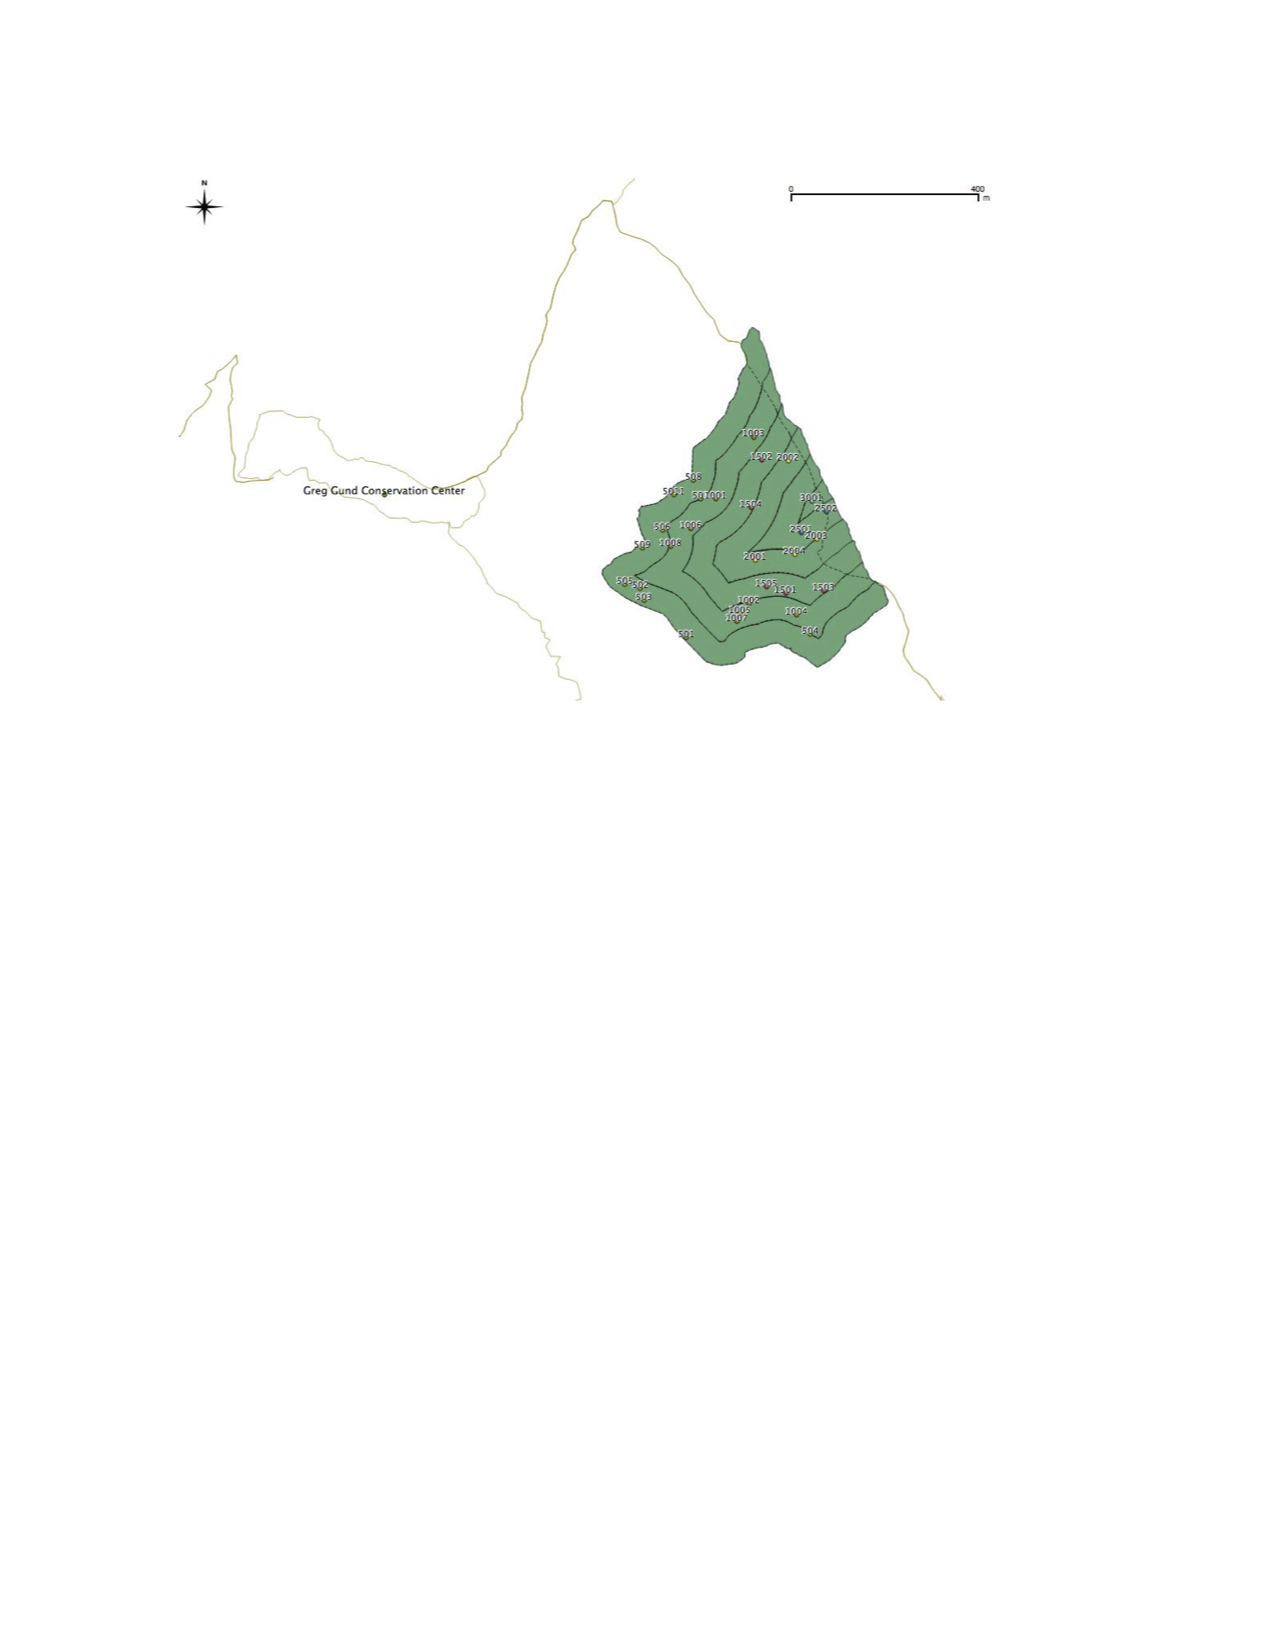
\includegraphics{../figs/map.png}

\hypertarget{iicensus-measurements}{%
\section{II--Census measurements}\label{iicensus-measurements}}

\begin{itemize}
\item
  Stems ≥10 cm were measured for DBH and height using rangefinder
  \emph{(Bushnell, Forestry Suppliers, Inc)}
\item
  Taxa were ID'd with help from local field guides
\item
  Plot canopy closure was measured with densiometer
\end{itemize}

\hypertarget{iistatistical-analysis}{%
\section{II--Statistical analysis}\label{iistatistical-analysis}}

\begin{itemize}
\item
  For all variables--

  \begin{itemize}
  \tightlist
  \item
    Trend lines follow median values of all plots in distance stratum
  \end{itemize}
\item
  Traits obtained from literature and compared to TRY database
  \emph{(Kattge and Str 2019)}
\item
  Computations done with R 4.1.3 depending on \emph{BIOMASS} 2.1.7,
  \emph{vegan} 2.5.7, and \emph{tidyverse} 1.3.1 packages
\end{itemize}

\hypertarget{iiistand-regeneration}{%
\section{III--Stand regeneration}\label{iiistand-regeneration}}

\begin{itemize}
\item
  Further from primary forest edge--

  \begin{itemize}
  \item
    Biomass and wood density tended to increase
  \item
    Stem density decreased then increased
  \item
    Neither canopy light nor height (not shown) tended to change
  \end{itemize}
\item
  Distance from forest edge tended to explain variation--

  \begin{itemize}
  \item
    10\% in wood density
  \item
    \textasciitilde20\% in stem density
  \end{itemize}
\end{itemize}

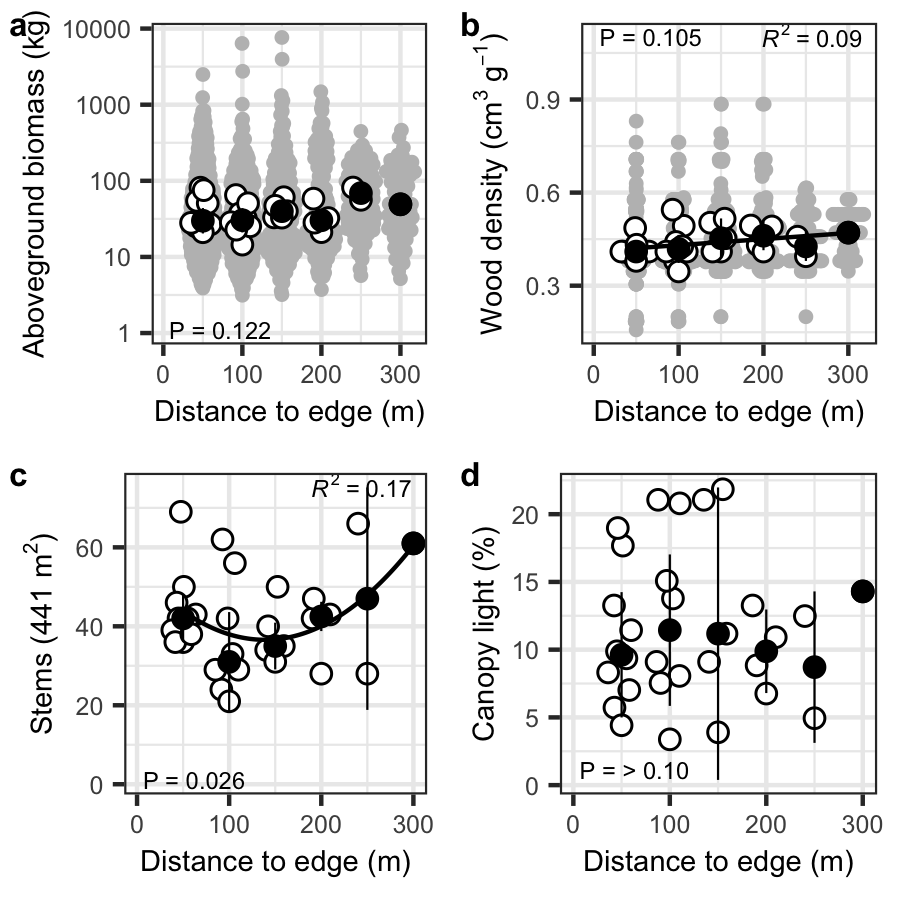
\includegraphics{../figs/fig1.png}

\hypertarget{iiicomposition-regeneration}{%
\section{III--Composition
regeneration}\label{iiicomposition-regeneration}}

\begin{itemize}
\item
  Further from forest edge--

  \begin{itemize}
  \item
    Richness tended to increase
  \item
    Diversity decreased steeply
  \item
    Composition varied notably, toward PC1
  \item
    Of abundant taxa biomass--

    \begin{itemize}
    \item
      Vochysia tended to decrease
    \item
      Ficus decreased
    \end{itemize}
  \end{itemize}
\end{itemize}

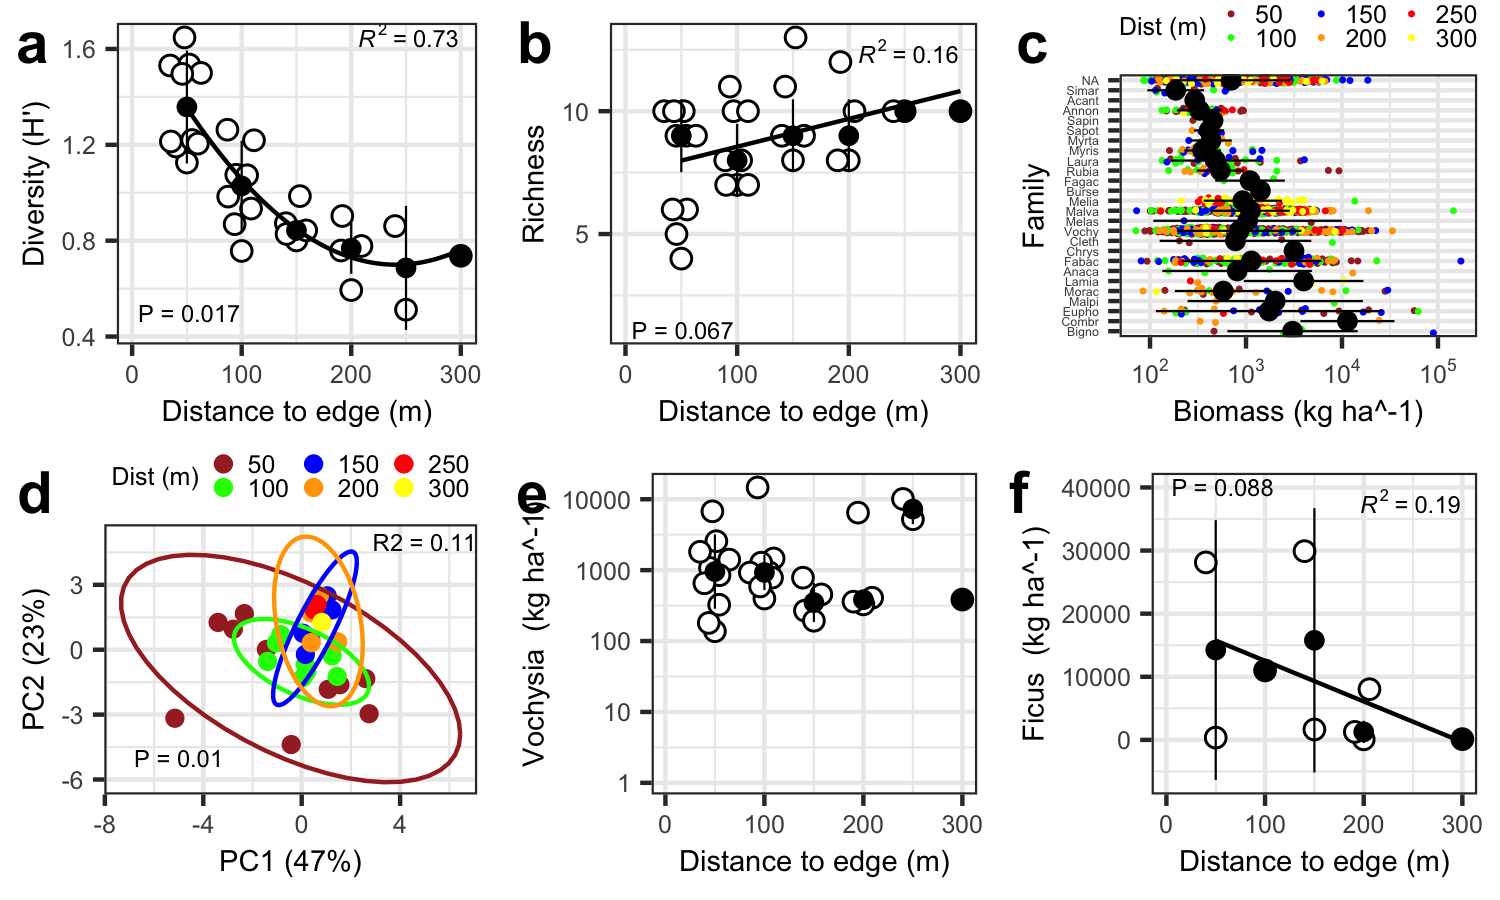
\includegraphics{../figs/fig2.png}

\hypertarget{iiifunctional-regeneration}{%
\section{III--Functional
regeneration}\label{iiifunctional-regeneration}}

\begin{itemize}
\item
  Away from forest edge--

  \begin{itemize}
  \item
    Biomass of taxa often found in both successional stages decreased
  \item
    Biomass based on dispersal mode remained constant
  \end{itemize}
\end{itemize}

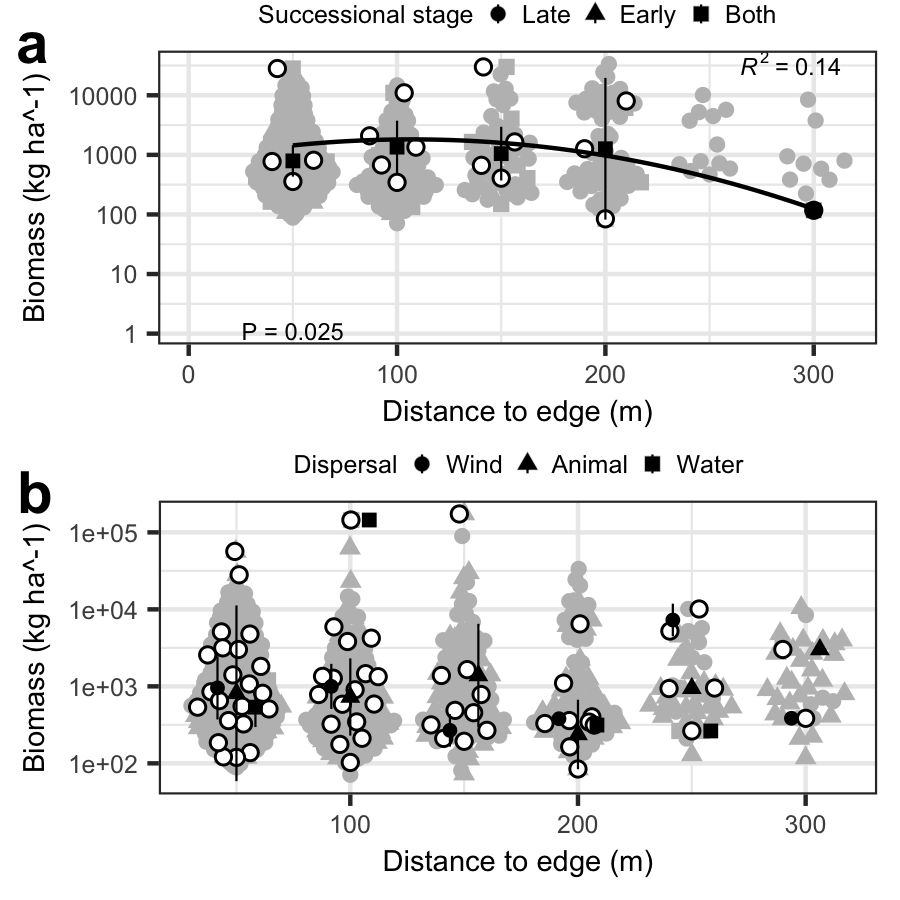
\includegraphics{../figs/fig3.png}

\hypertarget{ivhypothesis-check}{%
\section{IV--Hypothesis check}\label{ivhypothesis-check}}

\begin{itemize}
\item
  Stand biomass is more resilient than biodiversity

  \begin{itemize}
  \item
    Further from forest--

    \begin{itemize}
    \item
      No trends in biomass
    \item
      Diversity decreased
    \item
      Composition tended to change
    \end{itemize}
  \end{itemize}
\item
  Forest edge associated with tree diversity
\end{itemize}

\hypertarget{ivprocesses-underlying-patterns}{%
\section{IV--Processes underlying
patterns}\label{ivprocesses-underlying-patterns}}

\begin{itemize}
\item
  Not shade, perhaps given high absolute value and/or evenness of
  original timber planting
\item
  Forest edge may associate with faster succession, given drop in
  generalist tree taxa with distance
\item
  No signal of dispersal mode detected
\end{itemize}

\hypertarget{ivcompare-to-similar-studies}{%
\section{IV--Compare to similar
studies}\label{ivcompare-to-similar-studies}}

\begin{itemize}
\item
  Aligns well with several recent studies suggesting that--

  \begin{itemize}
  \item
    Tree diversity regenerates quicker than taxonomic composition
    \emph{(Poorter et al. 2016)}
  \item
    Habitat edges lower diversity and generally slow regeneration, like
    via less seed consumption \emph{(Hohlenwerger, Tambosi, and Metzger
    2022)}
  \item
    Taxa indiscriminate to successional stage are minimally affected by
    disturbance, like from edges \emph{(Bongers et al. 2009)}
  \end{itemize}
\end{itemize}

\hypertarget{ivfuture-studies}{%
\section{IV--Future studies}\label{ivfuture-studies}}

\begin{itemize}
\item
  Compare wet tropical plantations at different stages of regeneration
\item
  Compare forests with different initial composition but in similar
  region (i.e.~realized vs.~fundamental niches)
\item
  Study ecological dynamics under various management conditions
\end{itemize}

\hypertarget{references}{%
\section{References}\label{references}}

\hypertarget{refs}{}
\begin{CSLReferences}{1}{0}
\leavevmode\vadjust pre{\hypertarget{ref-bongers09}{}}%
Bongers, Frans, Lourens Poorter, William D. Hawthorne, and Douglas
Sheil. 2009. {``The Intermediate Disturbance Hypothesis Applies to
Tropical Forests, but Disturbance Contributes Little to Tree
Diversity.''} \emph{Ecology Letters} 12 (8): 798--805.
\url{https://doi.org/10.1111/j.1461-0248.2009.01329.x}.

\leavevmode\vadjust pre{\hypertarget{ref-haddad15}{}}%
Haddad, Nick M., Lars A. Brudvig, Jean Clobert, Kendi F. Davies, Andrew
Gonzalez, Robert D. Holt, Thomas E. Lovejoy, et al. 2015. {``Habitat
Fragmentation and Its Lasting Impact on {Earth}'s Ecosystems.''}
\emph{Science Advances} 1 (2): e1500052.
\url{https://doi.org/10.1126/sciadv.1500052}.

\leavevmode\vadjust pre{\hypertarget{ref-hohlenwerger22}{}}%
Hohlenwerger, Camila, Leandro Reverberi Tambosi, and Jean Paul Metzger.
2022. {``Forest Cover and Proximity to Forest Affect Predation by
Natural Enemies in Pasture and Coffee Plantations Differently.''}
\emph{Agriculture, Ecosystems \& Environment} 333 (August): 107958.
\url{https://doi.org/10.1016/j.agee.2022.107958}.

\leavevmode\vadjust pre{\hypertarget{ref-kattge19}{}}%
Kattge, Jens, and Hans Knöll Str. 2019. {``{TRY} Plant Trait Database
\textendash{} Enhanced Coverage and Open Access,''} 70.

\leavevmode\vadjust pre{\hypertarget{ref-norden15}{}}%
Norden, Natalia, Héctor A. Angarita, Frans Bongers, Miguel
Martínez-Ramos, Iñigo Granzow-de la Cerda, Michiel van Breugel, Edwin
Lebrija-Trejos, et al. 2015. {``Successional Dynamics in {Neotropical}
Forests Are as Uncertain as They Are Predictable.''} \emph{Proceedings
of the National Academy of Sciences} 112 (26): 8013--18.
\url{https://doi.org/10.1073/pnas.1500403112}.

\leavevmode\vadjust pre{\hypertarget{ref-poorter16}{}}%
Poorter, Lourens, Frans Bongers, T. Mitchell Aide, Angélica M. Almeyda
Zambrano, Patricia Balvanera, Justin M. Becknell, Vanessa Boukili, et
al. 2016. {``Biomass Resilience of {Neotropical} Secondary Forests.''}
\emph{Nature} 530 (7589): 211--14.
\url{https://doi.org/10.1038/nature16512}.

\leavevmode\vadjust pre{\hypertarget{ref-poorter21}{}}%
Poorter, Lourens, Dylan Craven, Catarina C. Jakovac, Masha T. van der
Sande, Lucy Amissah, Frans Bongers, Robin L. Chazdon, et al. 2021.
{``Multidimensional Tropical Forest Recovery.''} \emph{Science} 374
(6573): 1370--76. \url{https://doi.org/10.1126/science.abh3629}.

\leavevmode\vadjust pre{\hypertarget{ref-rozendaal19}{}}%
Rozendaal, Danaë M. A., Frans Bongers, T. Mitchell Aide, Esteban
Alvarez-Dávila, Nataly Ascarrunz, Patricia Balvanera, Justin M.
Becknell, et al. 2019. {``Biodiversity Recovery of {Neotropical}
Secondary Forests.''} \emph{Science Advances} 5 (3).
\url{https://doi.org/10.1126/sciadv.aau3114}.

\end{CSLReferences}

\end{document}
